% to-do
% -----
% - fill out data section
% - fill out method section
% - decide on best ``functional tests'' to convince any skeptical reader
% - choose examples

\documentclass[12pt,preprint,pdftex]{aastex}
\newcounter{address}
\newcommand{\foreign}[1]{\emph{#1}}
\newcommand{\etal}{\foreign{et~al.}}
\newcommand{\project}[1]{\textsl{#1}}
\newcommand{\documentname}{\textsl{Article}}
\newcommand{\sectionname}{Section}
\newcommand{\sectionnames}{\sectionname s}
\newcommand{\units}[1]{\mathrm{#1}}
\renewcommand{\mag}{\units{mag}}
\renewcommand{\arcmin}{\units{arcmin}}
\newcommand{\rfifty}{r_{50}}
\newcommand{\rninety}{r_{90}}
\newcommand{\conc}{C}

\begin{document}
\title{
       Measuring galaxies with very large angular sizes.
      }
\author{
        David Mykytyn\altaffilmark{\ref{CCPP}},
        Dustin Lang\altaffilmark{\ref{CMU}},
        Ekta Patel\altaffilmark{\ref{CCPP}},
        David W. Hogg\altaffilmark{\ref{CCPP},\ref{MPIA},\ref{email}}
       }
\setcounter{address}{1}
\altaffiltext{\theaddress}{\stepcounter{address}\label{CCPP} Center
  for Cosmology and Particle Physics, Department of Physics, New York
  University, 4 Washington Place, New York, NY 10003}
\altaffiltext{\theaddress}{\stepcounter{address}\label{CMU} Carnegie
  Mellon University}
\altaffiltext{\theaddress}{\stepcounter{address}\label{MPIA}
  Max-Planck-Institut f\"ur Astronomie, K\"onigstuhl 17, D-69117
  Heidelberg, Germany}
\altaffiltext{\theaddress}{\stepcounter{address}\label{email} To whom
  correspondence should be addressed: \texttt{david.hogg@nyu.edu}}

\begin{abstract}
The measurement of galaxies with large angular sizes is challenging,
and has rarely been done well in automated settings.  Issues include
that the galaxies overlap field boundaries, overlap foreground stars,
and show detailed and confusing internal structure at high
signal-to-noise.  We take a generative modeling or likelihood approach
to making measurements of the galaxies, using very simplified
few-parameter morphological models and with the likelihood modified
for robustness.  We show that we can get precise and reliable (though
possibly biased) measurements of colors and surface brightnesses for
very large galaxies ($>1~\arcmin$ in diameter) in the \project{Sloan
  Digital Sky Survey} imaging data.
\end{abstract}

\section{Introduction}

The \project{Sloan Digital Sky Survey} (\project{SDSS}) and its
successor projects \project{SDSS-II} and \project{SDSS-III} have had
enormous impact, forming the observational basis for literally
\emph{thousands} of refereed papers.  The success of these surveys can
be attributed to multiple factors, not least the unaccountable
diversity of phenomenology presented to us by our fecund Universe.
One significant factor has been the fact that these surveys have
endeavored to produce and distribute (to the public) reliable,
calibrated, easy-to-use photometric and spectroscopic data.

All that said, the goals of the \project{SDSS} were heavily weighted
towards galaxies and stars with visible brightnesses around 18~mag.
The camera, observing strategy, and data-reduction pipelines were all
optimized for performance at 15 to 22~mag.  Importantly---and to the
chagrin of some investigators (CITE SOMETHING)---the \project{SDSS}
photometry of very bright, nearby galaxies has been substantially
biased.  The dominant reason for this is that the \project{SDSS-I}
photometric pipelines employed an ``aggressive'' sky estimation
algorithm that removed much of the light from sources with large
angular footprints.  A secondary reason is that the ``deblending''
heuristics for disentangling the light in overlapping galaxies don't
deal well with sources that are hundreds or thousands of times the
solid angle of the core of the point-spread function.

The nearby galaxies are interesting and important!  Because the
\project{SDSS} is supremely well calibrated photometrically, and
because it is a drift-scanning survey, it is particularly well suited
to measuring these objects with large angular extents.  In this
\documentname, we make an attempt to photometer some nearby galaxies
in the \project{SDSS} imaging data and test the precision of those
measurements.

This project has been made possible by two developments.  The first is
that for \project{SDSS-III}, a new global, continuous sky function was
fit to the imaging data, fit to the ``blank'' pixels (CITE BLANTON).  This sky
function does not remove light from large galaxies, or not nearly as
much as previous generations of sky algorithms.  The second is that we
have developed a package \project{The Tractor} (HOGG CITE) for fitting
probabilistic models to astronomical imaging data and the
\project{SDSS} imaging in particular.

In what follows, we fit \project{SDSS} imaging
data on and near large angular-size galaxies using simple (inflexible)
models---mixtures of exponential and de~Vaucouleurs models.  For each
galaxy, we use \project{The Tractor} to
optimize a justifiable scalar objective function that is an
approximation to a likelihood, with modifications to make the fitting
less sensitive (than traditionally) to outliers and morphological
oddities in the galaxies.  The galaxies are typically as large as or
larger than an individual \project{SDSS} frame, but \project{The
  Tractor} doesn't need a co-add or mosaic of the data; it fits all
the individual disjoint science exposures simultaneously.  For most
galaxies we look at, the simple models we are using are \emph{not}
good fits: They can't be, because they don't capture spiral arms, HII
regions, dust lanes, or other morphological non-trivialities.
However, as we will show, they produce precise, robust photometry that
appears to be invariant with galaxy angular size or distance.

Readers who don't want to read the long philosophical position
outlined in \sectionname~\ref{sec:philosophy} can skip either to the
data and method descriptions in \sectionnames~\ref{sec:data} and
\ref{sec:method} or else straight to the results in
\sectionname~\ref{sec:results}.  There is a short final discussion in
\sectionname~\ref{sec:discussion}.

\section{Galaxy photometry is impossible}\label{sec:philosophy}

There is a deep sense in which obtaining precise and accurate galaxy
photometry is fundamentally impossible.  The reasons are multiple, but
the dominant reasons are, first, that the angular outskirts of
galaxies can contain significant luminosity but at incredibly low
surface brightness and unknown morphology, and secondly, that the
imaging point-spread function (PSF) can also have large-angle
contributions that are unknown.  The latter problem affects stellar
photometry also, but so long as the PSF is constant, precise and
accurate stellar photometry \emph{is} possible.  The difference
between galaxies and stars is that all point-like stars will
illuminate the PSF (correlate with it) identically.  Stellar
photometry does not rely on getting all this right so long as it deals
with it \emph{consistently} across stars.  Not so for galaxies, each
of which might have very different correlations with the PSF at large
angles.  There is no way to produce consistent photometry without
knowing things about every galaxy and every PSF that are---almost in
principle---unknowable.

These fundamental issues and also many pragmatic issues of noisy,
badly calibrated, and crowded imaging have forced astronomers to
consider many different methods for measuring galaxy fluxes.  Each has
flaws.  Here we give a highly biased and very brief review.
\begin{itemize}
\item Given digital imaging of a patch of sky that includes a galaxy,
  the simplest way to measure the flux of that galaxy is
  \emph{aperture photometry}.  This is the measurement of the total
  light (the integral of the intensity, found by summing pixel values)
  in the image above the sky (foreground and background) intensity
  within a fixed circular angular aperture, centered on the galaxy.
  This kind of photometry obtains different fractions of the galaxy
  light in galaxies that have different proper sizes or which lie at
  different radial (angular-diameter) distances; in this sense it
  doesn't produce photometry that is distance-independent.  It has
  many other problems as well, some of which will come up later in
  this list.
\item Aperture photometry can in principle be improved by scaling the
  radius of the aperture with the inverse radial (angular-diameter)
  distance to the galaxy.  This helps in making the photometry
  distance-independent, but it requires prior knowledge of the galaxy
  distances.  It also doesn't perfectly compensate for distance
  because galaxies at different distances but subject to the same (in
  angular size) PSF illuminate even the properly scaled apertures
  differently.  This change also doesn't account for galaxies with
  different proper sizes.
\item Aperture photometry can be made adaptive, adapting the aperture
  to the observed angular size of each galaxy.  This requires image
  analysis---galaxy size measurement---prior to the photometry.  In
  one extreme version, \emph{Isophotal photometry}, the photometric
  aperture is made the (usually very non-trivial) precise \emph{shape}
  of a particular intensity contour in the galaxy image.  Isophotal
  photometry is close to distance-independent for low-redshift
  galaxies; at high redshift relativistic intensity dimming
  ($[1+z]^{-4}$) breaks that symmetry.  Also, isophotal photometry
  will in general get very different fractions of the galaxy light
  from high and low surface-brightness galaxies.  It also remains at
  least slightly dependent on the PSF for the same reasons as the
  previous methods.
\item \emph{Petrosian photometry} \citep{petrosian} adapts the angular radius of
  the photometry aperture using a statistic of the galaxy profile that
  is insensitive to total surface brightness.  It works by identifying
  a radius at which the (azimuthally averaged) intensity is a fixed
  fraction of the mean within that radius.  Again, this method is at
  least slightly dependent on distance, again because of the PSF.
\item The most adaptive methods in common use---not the most adaptive
  \emph{possible}---involve measuring the galaxy's \emph{radial
    profile} by averaging the intensity above the sky intensity in
  narrow circular (or sometimes elliptical) annuli centered on the
  galaxy, and then summing the annular contributions to the flux, and
  maybe also extrapolating at large radius.  These methods are usually
  designed to attempt to get ``all the light''.  They do not overcome
  the fundamental problem of large-radius galaxy and PSF morphology.
\item One problem in common to all the above approaches is that they
  involve ``adding up'' the flux in pixels.  This arithmetic operation
  creates what is classically called a ``statistic'' of the data; it
  will not be the minimum-variance estimator of anything.  That is, if
  information preservation or precision is of high value, none of the
  above methods are palatable.  Information-preserving inference
  requires fitting probabilistic models, with a likelihood funtion at
  least and maybe also informative priors.  In the enormous
  \project{Sloan Digital Sky Survey}, despite the fact that aperture
  and Petrosian magnitudes were measured and published, it was the
  magnitudes based on \emph{model fitting} that got the most use: They
  produced more precise colors.  It is also the case that model
  fitting is the first method in this list that has a shot at
  producing truly distance-independent measurements, because a
  component of the model fit is the PSF.  Inasmuch as the galaxy and
  PSF models are appropriate and correct, model fitting is in some
  sense provably the best way to measure galaxy photometry.  Of course
  it doesn't overcome the fundamental problems of galaxy photometry
  with which this \documentname\ opens: We don't understand galaxy
  profiles or the PSF at large angular radii, and though there can be
  significant light out there, it is hard to find in the data.
  Furthermore, in the standard methodologies of model fitting,
  extremely simple galaxy models are used, such as elliptical
  exponentials and de~Vaucouleurs profiles \citep{dev}.  These smooth
  models are not at all a good description of two-dimensional images
  of most real galaxies at \emph{any} angular radius (think: spiral
  arms, bars, rings, HII regions, dust lanes, and so on).
\item An almost unexplored territory for galaxy photometry is to
  consider extremely flexible galaxy models, models so flexible that
  they can capture all of the details.  This would require a
  significant technical investment and a lot of computer time, but it
  might pay off.  It ought to give the best measurements in the end;
  it is the ultimate in ``letting the data decide''.  However, even
  this flexible approach won't overcome the fundamental problems; in
  some sense the true, total photometry of a galaxy is \emph{not an
    observable}.
\end{itemize}
All the problems with these different photometric measurement
techniques flow into the subsequent or simultaneous measurements made
of other quantities of interest, like sizes, concentrations, surface
brightnesses, and so-on, because these measurements are (or involve)
transformations of photometric measurements.  The best choice among
techniques will depend on the uses to which the measurements are going
to be put; in some cases precision is paramount, in others consistency
across distance, in others robustness to varying PSF, in others
consistency across morphological types.

In this project, our goal is to obtain consistent multi-band
photometry for a large set of galaxies at a wide range of distances,
with a large range of morphologies, surface-brightnesses, and angular
sizes relative to the PSF.  Importantly, we want to do the very
(angularly) large galaxies in the same way as we do the (angularly)
compact.  Consistency is more important than accuracy, in the sense
that we would like to get numbers that---if they must be wrong---are
wrong \emph{in the same way} for the \emph{same galaxy} observed at
different distances or through different atmospheric PSFs.  We also
want precision---we want to avoid introducing unnecessary scatter or
noise by our choice of procedure.

These considerations argue \emph{for} probabilistic modeling and
\emph{against} using very flexible models.  We are making a catalog of
photometry, not delivering posterior PDFs; our photometry will
therefore contain \emph{estimators} for flux, color, size, and so-on.
Minimum variance estimators are maximum-likelihood estimators, so we
will only consider approaches in which we (under assumptions)
construct an approximate likelihood function and optimize it.  As we
note above, the requirement that our photometry be distance and
PSF-independent also argues for modeling approaches.  The reason we
prefer inflexible models to flexible models is that at the optimum in
the likelihood, a large angular-size galaxy will exercise much more
model freedom than a small angular-size galaxy: In the large galaxy,
many more features and details are visible under finite PSF.  Again,
distance and PSF consistency requires that we restrict model freedom
identically or as identically as possible for all galaxies we measure.
This argues for overly simplistic models; the models we will use below
do \emph{not} capture the full two-dimensional structure of the
galaxies being measured, but (as we will show), they do provide
robust, high signal-to-noise, consistent measurements.

In addition to the photometric issues discussed above, there are a
large number of separate pragmatic issues when we consider the problem
of performing galaxy photometry automatically and consistently in a
large and heterogeneous data set.  When galaxies are angularly large,
as they will be here, they often overlap stars.  Bright stars make it
hard to precisely measure the fainter galaxy.  Faint stars are
challenging to deblend from the galaxy reliably.



In addition to overlapping stars, galaxies frequently overlap other
galaxies, both because galaxies are spatially clustered and because
some ``galaxies'' are really pairs of galaxies merging.  Overlapping
galaxies must be ``deblended'', which is a source of consternation in
many imaging surveys.  The consternaton arises both because proper
deblending is an ill-posed problem and because it is very
distance-dependent.  The problem is ill-posed because there is no
definition of the boundary between two galaxies and one; even if there
were, we wouldn't know how to separate the observed intensity into the
two components.  Clever data-driven heuristic proposals and methods
exist (cite Lupton and SExtractor) but nothing is reliable for
angularly large galaxies, where enormous non-smooth detail is visible
for a large range of Hubble types.  Deblending is distance-dependent,
because a galaxy observed nearby is much larger than the PSF; all of
the spiral structure and HII regions are well resolved.  A distant
galaxy is a smooth blob under the PSF.  The deblending simply can't be
the same if it is based on flexible heuristics.  This is another place
where fitting inflexible models will help us: Although the inflexible
models are never good fits, they provide objective methods for
simultaneously measuring two overlapping galaxies.

\section{Data and input catalogs}\label{sec:data}

The imaging data for this project come from the \project{Sloan Digital
  Sky Survey} fully public \project{Data Release 8} \citep{dr8}, which is
the first data release of the \project{SDSS-III} project \citep{sdssiii}.  It
includes fully recalibrated imaging \citep{padmanabhan} from the
combined imaging projects of \project{SDSS} \citep{york}  and
\project{SDSS-II} \citep{sdssii}.

...key point is the new sky...

The fitting code (\project{The Tractor}, described briefly below, and
more completely in Lang \etal, forthcoming) locates \project{SDSS}
imaging fields that overlap a large circular footprint centered on the
pre-fitting (input) galaxy center.  It downloads (on the fly)
\project{DR8} imaging data files corresponding to those fields from
the \project{SDSS-III} \project{Data Archive Server} (CITE?).  The
downloaded data files are the photometrically calibrated,
background-subtracted ``frames'' files.

For every pixel of the imaging, we construct an approximate ``inverse
variance'' value, which is the reciprocal of the variance expected
given the Poisson photon, Poisson dark-current, and Gaussian
read-noise error models.  In detail, we use the equations recommended
by the \project{SDSS-III}
Collaboration.\footnote{\url{http://data.sdss3.org/datamodel/files/BOSS\_PHOTOOBJ/frames/RERUN/RUN/CAMCOL/frame.html}}
We set the inverse variance to zero for any pixels that lie in regions
that were interpolated, saturated, or affected by cosmic rays or ghost
images.

For the PSF model, we use the SDSS double-Gaussian model stored in the
``psField'' file.  DSTN: What do we get as parameters for that
double-Gaussian model?  I think it is less than 1 + 4 + 6 parameters
that a K=2 D=2 MoG would have, right?

Galactic extinction $E(B-V)$ values are taken at the galaxy center
positions from the standard maps (\citealt{schlegel98}).  The
reddening values are then multiplied by the appropriate coefficients
A(V)/E(B-V) per Sloan bandpass to obtain the total extinction to be
subtracted from the individual magnitudes of each bandpass. The
coefficiens are the following: u-5.155,g-3.793, r-2.751, i-2.086,
z-1.479.

In this paper we use a sample of galaxies for testing which we do not
intend to be complete.  The source for this sample---which is only
really bringing initial (or first-guess) celestial positions---was the
Third Reference Catalog of Bright Galaxies \citep{rc3}.  From this
catalog we used only objects with angular diameter measured in the
apparent major isophotal diameter at the surface brightness level
$\mu_B = 25.0$~mag in 1~arcsec$^2$ arcsecond of [DM WHAT SYMBOL?]
$>1$~arcmin.

\section{Method}\label{sec:method}

...first a few words about \project{The Tractor}

Models: Write about the types of models used?? Different galaxies types etc?
The Tractor functions first by building a model, using initial parameter data that is supplied. Next, it takes the derivative of each parameter and performs a weighted least-squares fit to find a parameter update that will minimize $\chi^2$.  Since this is a linearization of a non-linear problem, we perform a line search along the update direction, taking steps of increasing size starting from $1/1024$ and increasing by factors of $2$ up to a factor of $2$ of the linear direction; we halt the line-search when the $\chi^2$ stops decreasing.  Finally the parameters are updated in that direction. The tractor is capable of freezing certain parameters, so that they are excluded from the optimization. 
The iteratively-reweighted least squares process is used to update the
inverse variances after each iteration of optimization. The math is:
\begin{eqnarray}
\chi^2 &\equiv& \sum_n \chi_n^2
\\
\chi_n^2 &\equiv& \frac{[d_n - m_n]^2}{\sigma_n^2}
\\
\frac{1}{\sigma_n^2} &\leftarrow& \frac{1}{\sigma_n^2}\,\frac{Q^2}{Q^2+\chi_n^2}
\quad ,
\end{eqnarray}
where $Q$ is the number of ``sigma'' at which the residual saturates. $Q$ for these fittings was chosen to be 5. (Find out why)

In order to deal with the problems of stars that overlap with the
galaxy which we are interested in, we decided to mask them out. The
stars were found using the data in the Tycho-2 star catalog \citep{tycho2}.
The stars were masked out to a
radius of
\begin{equation}
\theta_{\mathrm{exclude}} = \max(25, 25\,2^{[11\,\mag-V]})
\end{equation}
where $V$ is the visual magnitude given by Tycho-2.
(I'm not sure why these values, I got them from Dustin) The mask was applied by setting the chi values of the masked out pixels to zero.



...now the specifics of what we actually do

When given an RA and a Dec and a radius, the program searches the SDSS data for fields which overlap anywhere in that space. It downloads all those fields, in all bands, as fits files, and then imports them into the program as arrays. The initial inverse variances are also downloaded from Sloan.
Saturated pixels from the SDSS images were masked and then a binary dilation with three iterations was applied. (more details needed here?)

For the purpose of measuring and optimizing on a single galaxy at a
time, all other objects were removed from within a circle centered on
the galaxy center and radius, both given by the RC3 catalog (using the major isophotal diameter)
 for that particular catalog. This was done rather than
working within the SDSS catalog because SDSS frequently splits up large
galaxies into numerous small ones and so it was much easier to simply
start over with a single galaxy. As initialization, that galaxy was
given magnitudes of 15 in every band and a radius given by the RC3
catalog.


We start the fitting with an exponential galaxy and then optimize
simply that galaxy six times. Following that, we switch to a composite
galaxy, with both exponential and deVaucouleur components. These
components are free to vary separately in order to best fit the
data. This new composite galaxy is also optimized six times by itself.

In order to measure the half-light radius $\rfifty$, the 90 percent
radius $\rninety$ and the concentration parameter $\conc\equiv
\rninety/\rfifty$, we took the model of the galaxy that had been
optimized and places it in an empty frame within the tractor. Next,
over a series of increasing intervals of radii we summed up the total
flux within the circles and then interpolated to find $\rfifty$ and $\rninety$.
 We used sixty-four radii equally spaced in pixel logarithms from zero
 to half the height of the image. Exceptional cases were flagged for later
 review if $\rfifty$ was not between the deVaucouleur and exponential radii
 for that galaxy, and concentration was flagged as incorrect if $\frac{1}{\conc}$
 was not between .29 and .46. (We are not getting these numbers, mention in
 discussion?) TODO: Add citation to paper for these numbers.

An example of the finished result is given for NGC 4605, which had 6 fields that combined to make our image. These six are shown separately here. In fig \ref{fig:4605data} the data from these fields are shown in the i-band. Fig \ref{fig:4605model} shows our completed model for this galaxy. Fig \ref{fig:4605diff} is the difference between the data and the model. Finally \ref{fig:4605chi} shows our chi values for the galaxy. Fig \ref{fig:colorsdata} shows the different data for each band, and figs \ref{fig:colorsmodel}, \ref{fig:colorsdiff}, \ref{fig:colorschi} shows the results for the model, the difference between the model and the data, and the chi values.





\section{Exceptions and issues}\label{sec:results}
For instance, the galaxy M81 had too large of a radius in RC3 in order to run properly so it was manually reduced so as to fit into the memory of the machine. The scaling factors used were if the number of fields were between ten and twenty, a factor of two scaling. Four was used for between twenty and forty, and eight was used for between forty and eighty. Above eighty, the galaxy was skipped. (Put into table?) Another example is M51a and M51b, which were simultaneously fit in order to ensure that the fit measured both galaxies simultaneously. 

An example of two galaxies that were fit together and succeeded is fig \ref{fig:gooddouble} which shows the fit for NGC 3395 and NGC 3396. A bad fit of two galaxies is shown in fig \ref{fig:baddouble} of NGC 4647 and NGC 4649. In addition, fig \ref{fig:badsingle} shows an attempt to fit UGC 5613, which fails because it is actually composed of two merging galaxies.

Another common error cause is edge-on galaxies, as shown in fig \ref{fig:edgeon} which shows the failure of a fit of edge-on galaxy NGC 5907. 

All data that was flagged for review was reviewed by examination of the flipbook for that galaxy, in order that changes could be made to the initialization for that galaxy, or if the expected galaxy was nonexistent and therefore a mistake in a prior catalog, removed entirely from the catalog. 


\section{Discussion}\label{sec:discussion}
Precision of colors...

\acknowledgements It is a pleasure to thank
  Jim Gunn (Princeton),
  Robert Lupton (Princeton), and
  David Spergel (Princeton)
for valuable discussions.
This work was supported in part by The Princeton University Press,
NASA (grant NNX12AI50G) and the NSF (grant IIS-1124794).

...HOGG: Insert relevant SDSS boilerplate here...

\begin{thebibliography}{70}
\bibitem[Aihara \etal(2011)]{dr8}
Aihara, ~H., 2011, The Astrophysical Journal Supplement \volume{193}(2), article 29
\bibitem[de~Vaucouleurs(1948)]{dev}
de~Vaucouleurs,~G., 1948, Annales d'Astrophysique, 11, 247
\bibitem[de Vaucouleurs (1991)]{rc3}
de Vaucouleurs, ~G., de Vaucouleurs,~A., Corwin, ~H.~G., Buta, ~R.~J., Paturel, ~G., Fouqu\'{e}, ~P., 1991, Volume I
\bibitem[Eisenstein \etal(2011)]{sdssiii}
Eisenstein, ~D., 2011. \aj~142, 72 
\bibitem[Frieman \etal(2008)]{sdssii} %Not sure if this is correct sdss-ii paper
Frieman, ~J., 2008. \aj~135, 338
\bibitem[H\o{}g \etal(2000)]{tycho2}
H\o{}g,~E. \etal, 2000, \aap 335, L27
\bibitem[Lupton, \etal(2001)]{lupton}
Lupton, ~R., 2001. ASP Conf. Ser. 10, 269
\bibitem[Padmanabhan \etal(2008)]{padmanabhan}
Padmanabhan, ~N.,2008, \apj~135, 10-19
\bibitem[Petrosian(1976)]{petrosian}
Petrosian, ~V., 1976. Astrophysical Journal, 209, L1 %Not sure if this is the right way to cite this journal
\bibitem[Schlegel \etal(1998)]{schlegel98}
Schlegel,~D.~J., Finkbeiner,~D.~P., Davis,~M., \apj~500, 525
\bibitem[York \etal(2000)]{york}
York, D.~G., 2000, \aj~120, 1579
\end{thebibliography}

\begin{figure}
\centering
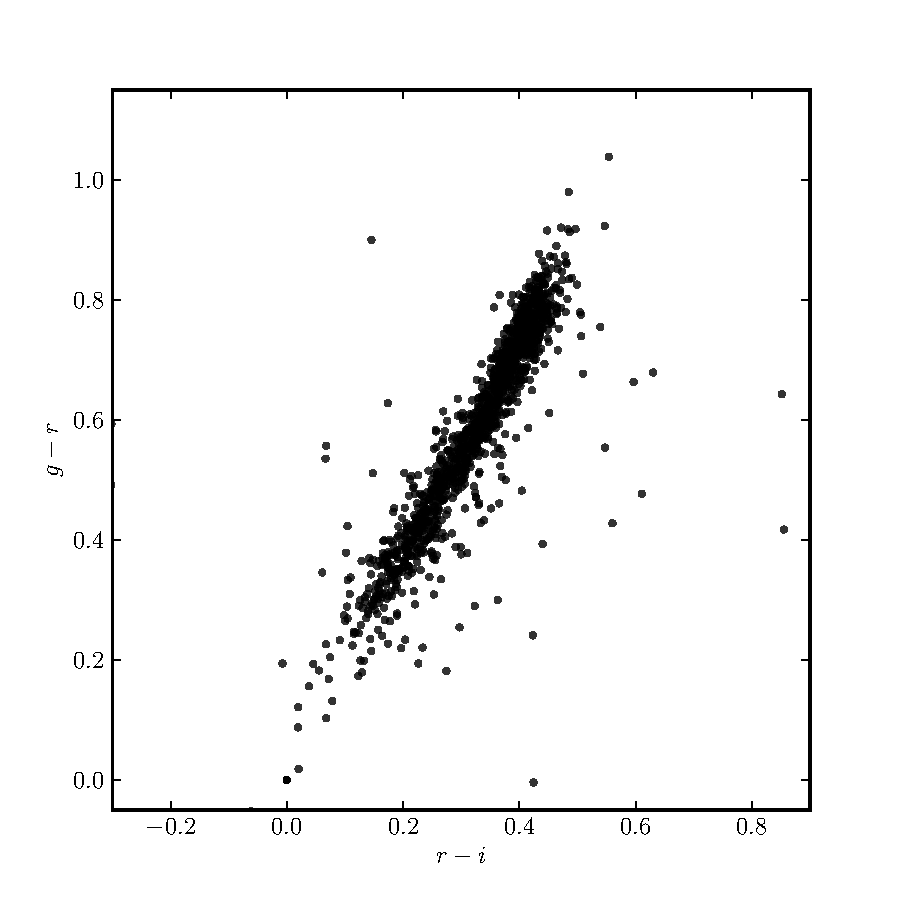
\includegraphics[trim = 15mm 0mm 0mm 0mm]{method_color_sloan.pdf}
\caption{A color-color plot of our Sloan Atlas data}
\end{figure}

\begin{figure}
\centering
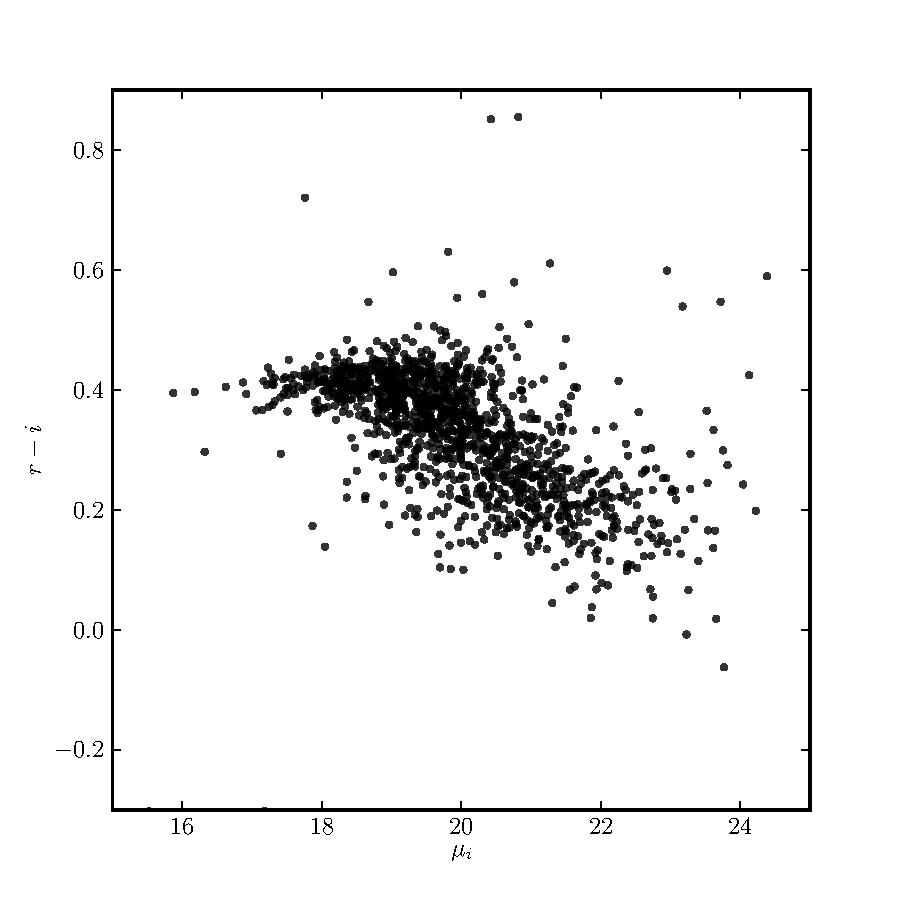
\includegraphics[trim = 15mm 0mm 0mm 0mm]{method_sb2_sloan.pdf}
\caption{Surface brightness in the i-band versus the r-i color for our Sloan Atlas data}
\end{figure}

\begin{figure}
\centering
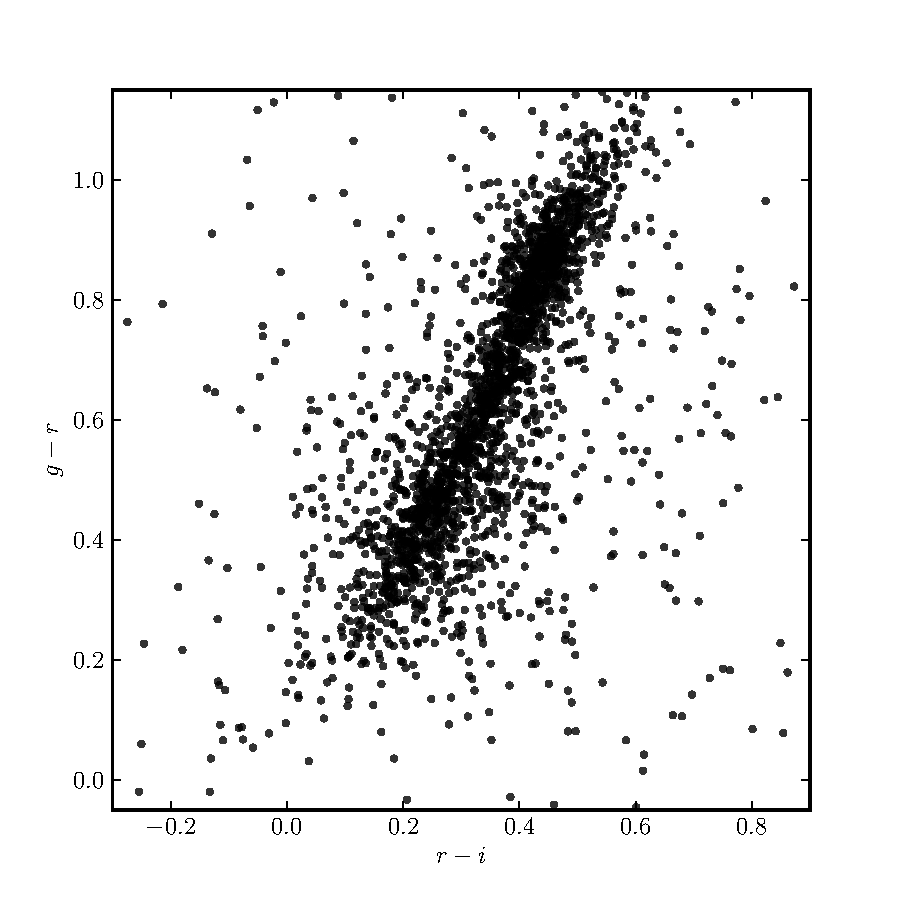
\includegraphics[trim = 15mm 0mm 0mm 0mm]{method_color_nsa.pdf}
\caption{A color-color plot of the NASA-Sloan Atlas data}
\end{figure}

\begin{figure}
\centering
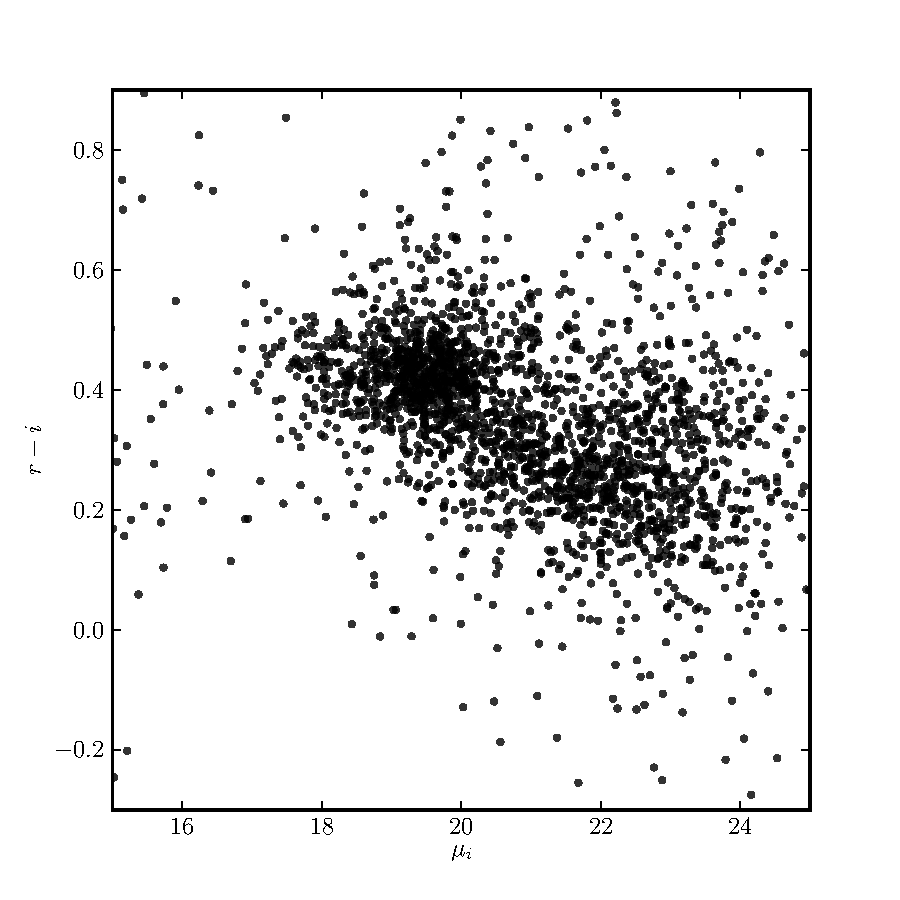
\includegraphics[trim = 15mm 0mm 0mm 0mm]{method_sb2_nsa.pdf}
\caption{Surface brightness in the i-band versus the r-i color for the NASA-Sloan Atlas data}
\end{figure}

\begin{figure}
\centering
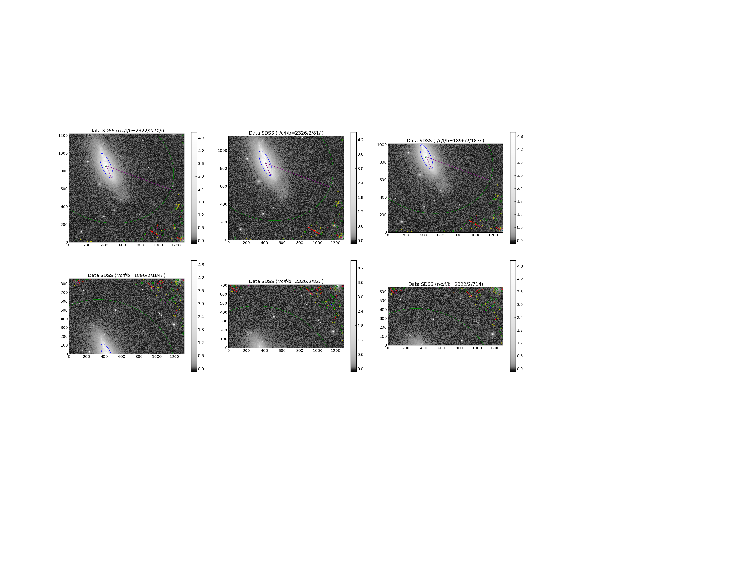
\includegraphics[trim = 1cm 3.2cm 3.8cm 2.15cm,clip=true,width=\textwidth] {data.pdf}
\caption{This shows the six different fields of data which are combined for the galaxy NGC 4605. The different fields represent different images taken by the Sloan telescope at different positions and different times.}
\label{fig:4605data}
\end{figure}
\begin{figure}
\centering
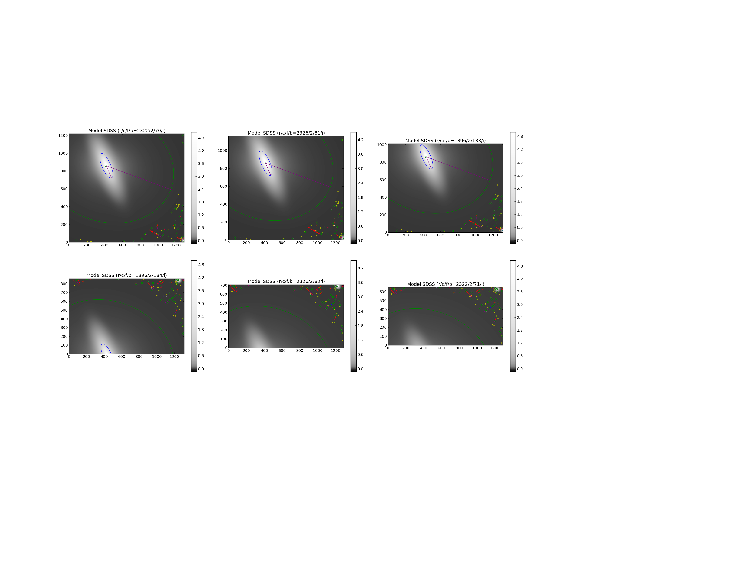
\includegraphics[trim = 1cm 3.2cm 3.8cm 2.15cm,clip=true,width=\textwidth] {model.pdf}
\caption{This is like fig \ref{fig:4605data} but shows the model we have built for the galaxy}
\label{fig:4605model}
\end{figure}
\begin{figure}
\centering
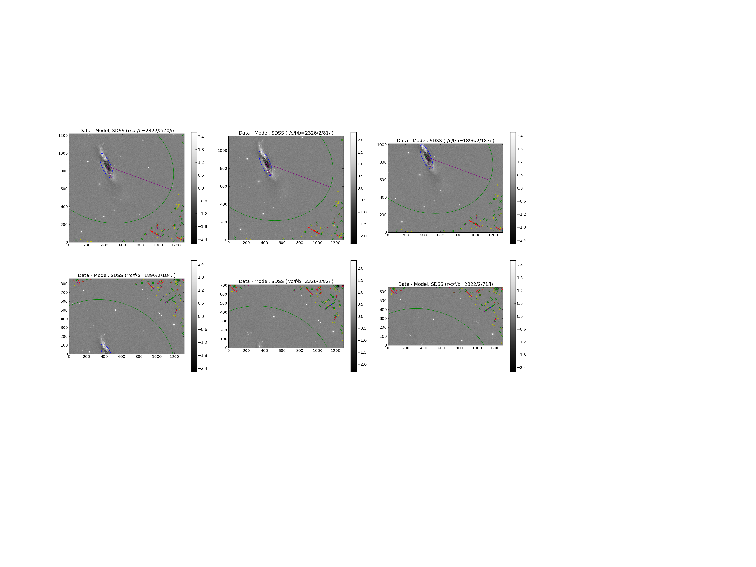
\includegraphics[trim = 1cm 3.2cm 3.8cm 2.15cm,clip=true,width=\textwidth] {diff.pdf}
\caption{This figure shows the difference between fig \ref{fig:4605data} and fig \ref{fig:4605model}}
\label{fig:4605diff}
\end{figure}
\begin{figure}
\centering
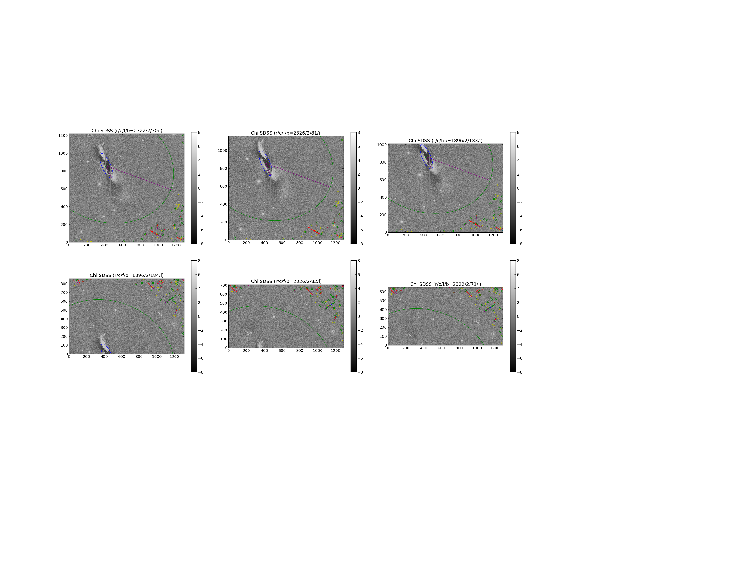
\includegraphics[trim = 1cm 3.2cm 3.8cm 2.15cm,clip=true,width=\textwidth] {chi.pdf}
\caption{This is the same as fig \ref{fig:4605diff} but shows the chi values, meaning that some pixels are masked out if they contain bad data.}
\label{fig:4605chi}
\end{figure}
\begin{figure}
\centering
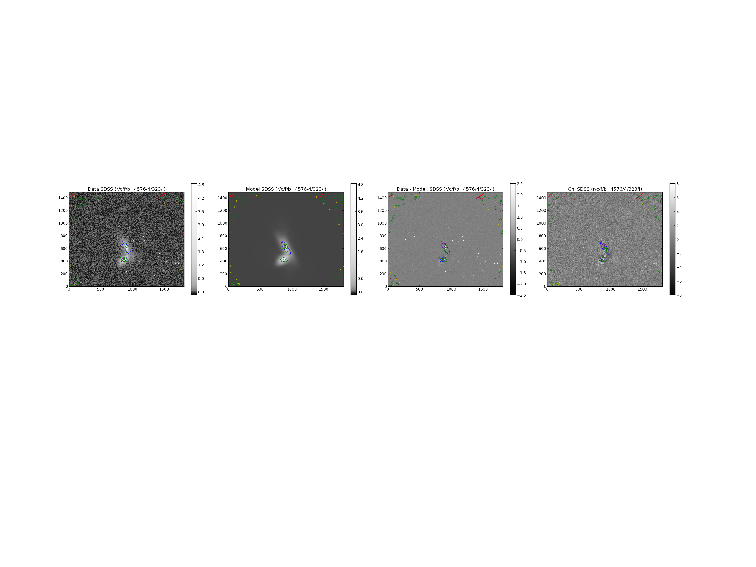
\includegraphics[trim = .9cm 4.5cm 1.15cm 2.9cm,clip=true,width=\textwidth] {gooddouble.pdf}
\caption{This figure show the fit for the galaxies NGC 3395 and NGC 3396, which are fit simultaneously. From left to right, this shows the data, the model, the residues, and the chi values in just one of the fields.}
\label{fig:gooddouble}
\end{figure}
\begin{figure}
\centering
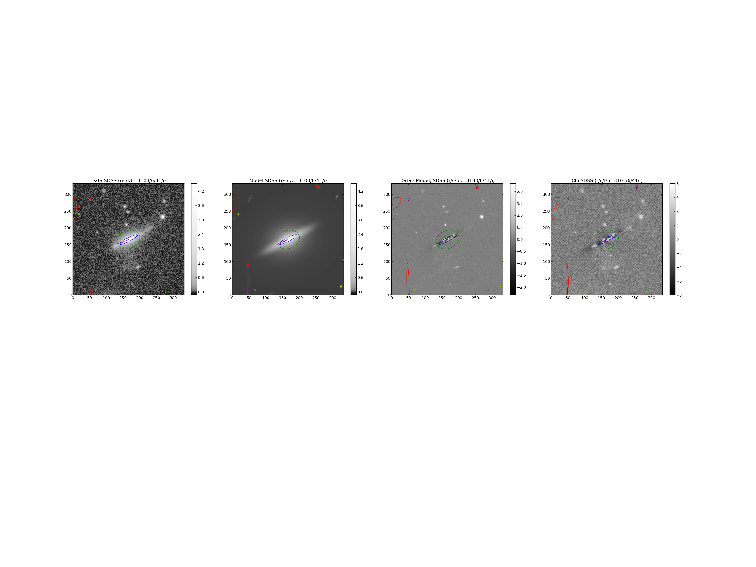
\includegraphics[trim = .9cm 4.5cm 1.15cm 2.9cm,clip=true,width=\textwidth] {badsingle.pdf}
\caption{This figure show the fit for the galaxy UGC 5613. This fit is bad because it fails to take into account that UGC 5613 is composed of a merger of two different galaxies, which causes our fit to fail. From left to right, this shows the data, the model, the residues, and the chi values in just one of the fields.}
\label{fig:badsingle}
\end{figure}
\begin{figure}
\centering
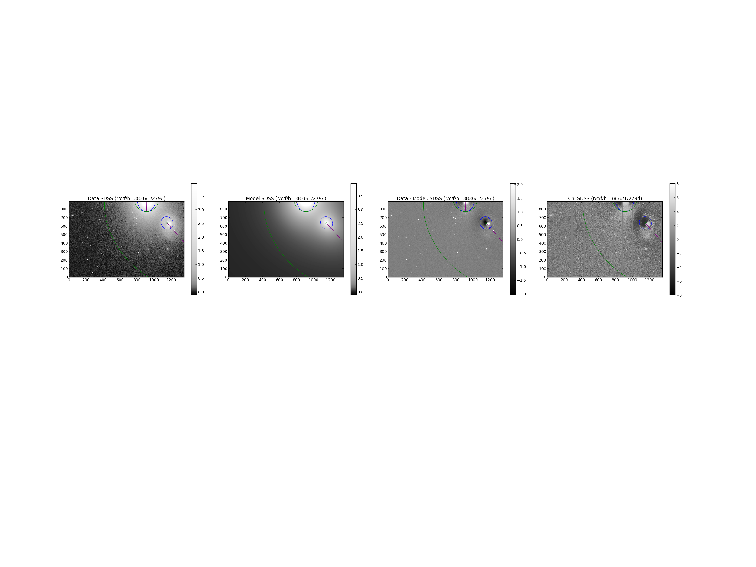
\includegraphics[trim = .9cm 4.5cm 1.15cm 2.9cm,clip=true,width=\textwidth] {baddouble.pdf}
\caption{This figure show the fit for the galaxies NGC 4647 and NGC 4649. This example shows a failure of the attempt to fit two galaxies simultaneously. From left to right, this shows the data, the model, the residues, and the chi values in just one of the fields.}
\label{fig:baddouble}
\end{figure}
\begin{figure}
\centering
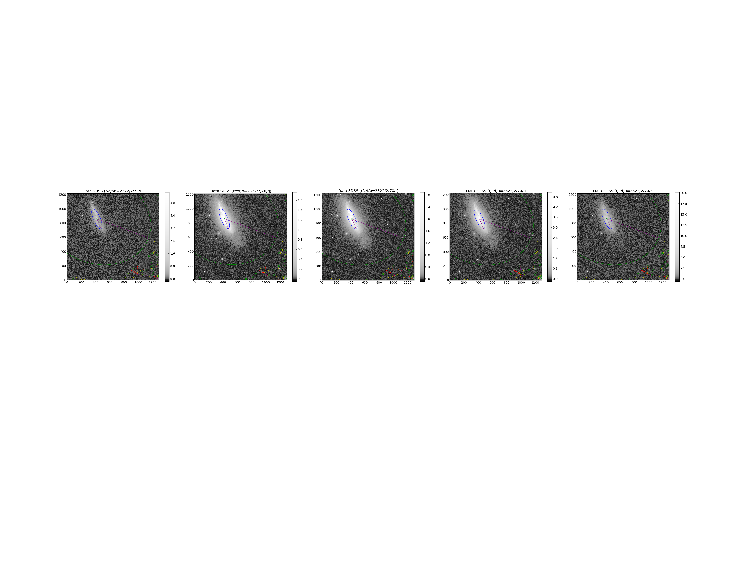
\includegraphics[trim = .9cm 4.5cm 0cm 2.9cm,clip=true,width=\textwidth] {goodsingle-colors-data.pdf}
\caption{This figure show the data for the five different bands for NGC 4605.}
\label{fig:colorsdata}
\end{figure}
\begin{figure}
\centering
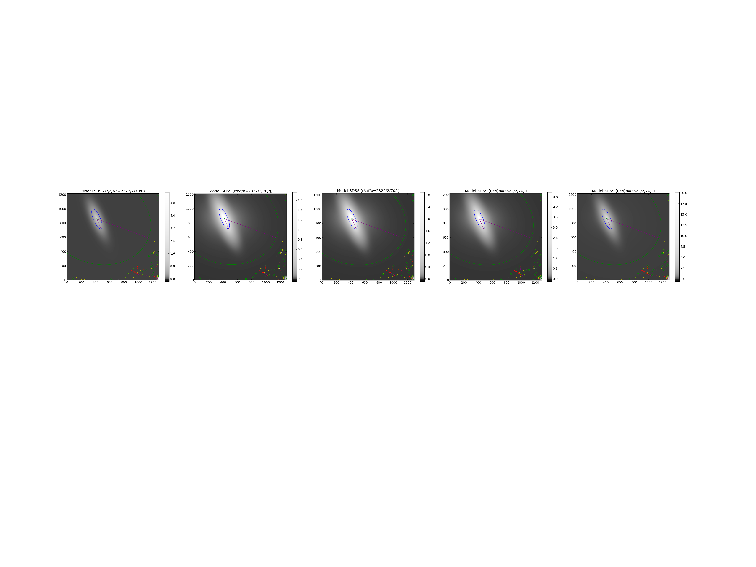
\includegraphics[trim = .9cm 4.5cm 0cm 2.9cm,clip=true,width=\textwidth] {goodsingle-colors-model.pdf}
\caption{This figure show the model for the five different bands for NGC 4605.}
\label{fig:colorsmodel}
\end{figure}
\begin{figure}
\centering
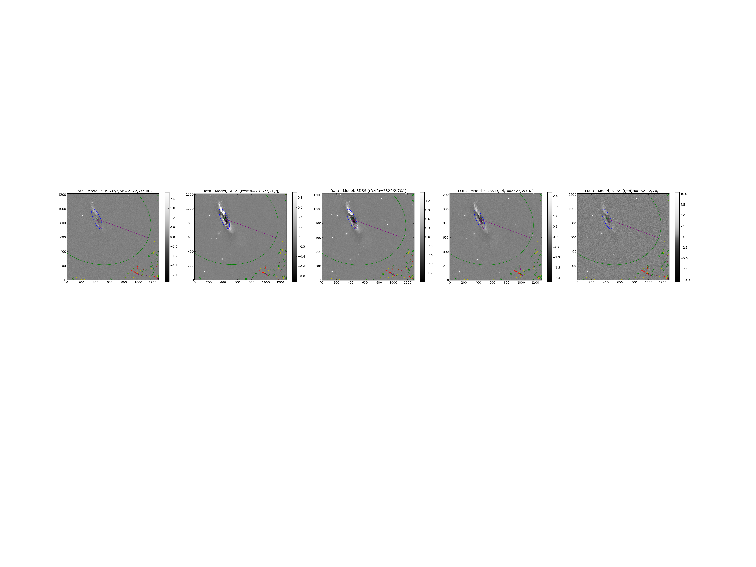
\includegraphics[trim = .9cm 4.5cm 0cm 2.9cm,clip=true,width=\textwidth] {goodsingle-colors-diff.pdf}
\caption{This figure show the diff for the five different bands for NGC 4605.}
\label{fig:colorsdiff}
\end{figure}
\begin{figure}
\centering
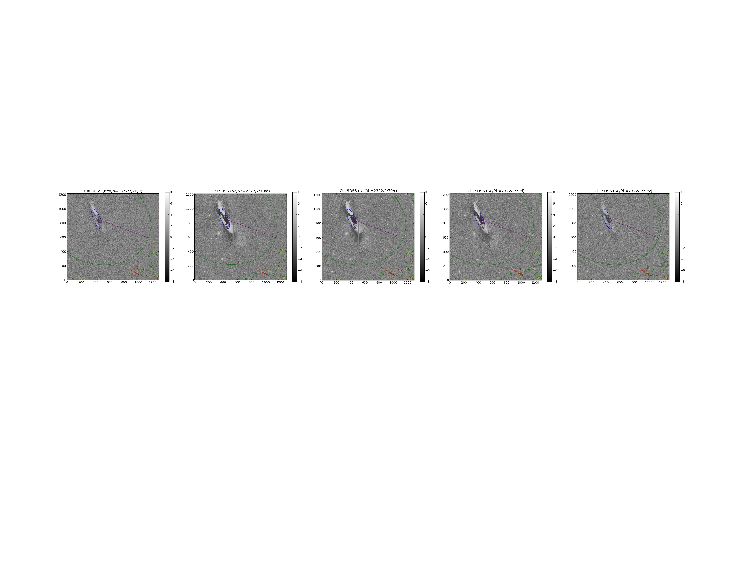
\includegraphics[trim = .9cm 4.5cm 0cm 2.9cm,clip=true,width=\textwidth] {goodsingle-colors-chi.pdf}
\caption{This figure show the chi for the five different bands for NGC 4605.}
\label{fig:colorschi}
\end{figure}
\begin{figure}
\centering
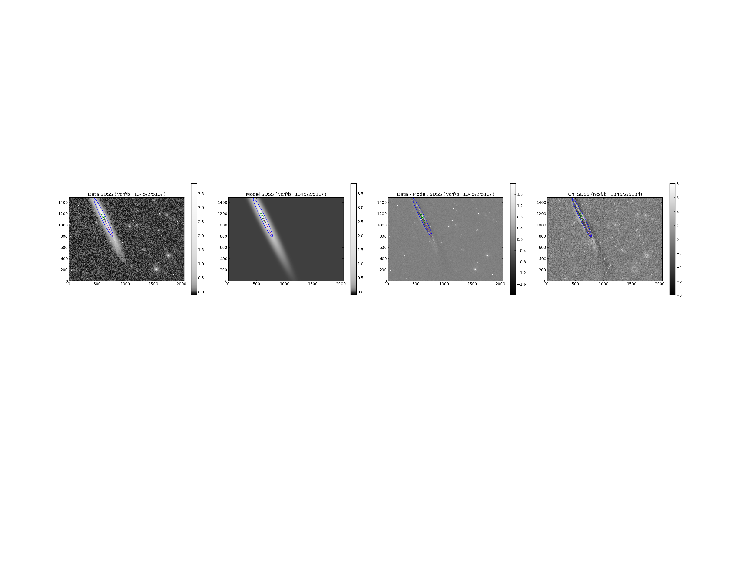
\includegraphics[trim = .9cm 4.5cm 1.15cm 2.9cm,clip=true,width=\textwidth] {edgeon.pdf}
\caption{This figure show the fit for the galaxy NGC 5907. This fit is bad because it fails on edge-on galaxies. From left to right, this shows the data, the model, the residues, and the chi values in just one of the fields.}
\label{fig:edgeon}
\end{figure}









\end{document}
